\section{Linear Regression using {Desmos}}

\gap{Linear} \gap{regression} is a mathematical way to automatically find the 
line of best fit.
The results tell you 
\begin{itemize}[nosep]
    \item the \gap{equation} of the line of best fit 
        \begin{itemize}[nosep]
            \item slope: \gap{$m$}
            \item $y$-intercept: \gap{$b$} 
            \item equation of the line: \gap{$y=mx+b$}
        \end{itemize}
    \item how well the line \gap{fits} the data in the scatterplot
        \begin{itemize}
            \item correlation coefficient: \gap{r}
        \end{itemize}
        \begin{center}
            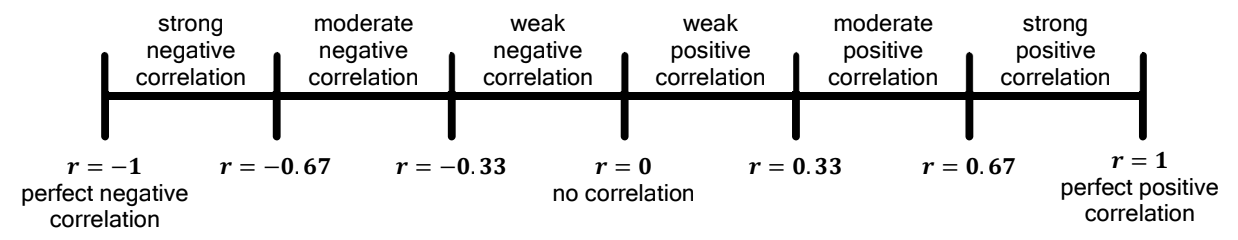
\includegraphics[height=1.1in]{correlation-strengths.png}
        \end{center}
\end{itemize}

\begin{myConcept}{To find the line of best fit using {\scshape Desmos}\dots}
    \begin{enumerate}[]
        \item Open the {\scshape Desmos Graphing Calculator} on your phone or laptop.
        \item Enter the $(x,y)$ data.
            \begin{itemize}
                \item Click 
                    \raisebox{-0.5em}{
\includegraphics[width=0.25in]{plus-button.png}}
                    in the upper left corner.
                \item Select \gap{``table''} to get an $(x_1,y_1)$ table for your data.
                \item Enter all the \gap{$x$} and \gap{$y$} values into the table.
            \end{itemize}
        \item Set up the window so you can see all the points.
            \begin{itemize}
                \item Click 
                    \raisebox{-0.5em}{
\includegraphics[width=0.3in]{wrench-tool.png}} 
                    in the upper right corner.
                \item Under \gap{\ttfamily X-Axis}, enter the low/high bounds of $x$ values to display.
                \item Under \gap{\ttfamily Y-Axis}, enter the low/high bounds of $y$ values to display.
            \end{itemize}
        \item Look at the scatterplot. You should see dots for your data.
        \item Do the linear regression.
            \begin{itemize}
                \item Tap the line \myEmph{below} the table.
                \item Enter \gap{$y_1 \thicksim m x_1 + b$}
                    \quad (Remember that \fbox{$\thicksim$} is on the {\ttfamily ABC} keypad.) 
            \end{itemize}
        \item {\scshape Desmos} shows you the values of
            \begin{itemize}
                \item \gap{$m$} and \gap{$b$} (slope and $y$-intercept of the line of best fit)
                \item The \gap{graph} of the \gap{line} of \gap{best} \gap{fit} in the scatterplot.
                \item \gap{$r$} (the correlation coefficient)
            \end{itemize}
    \end{enumerate}
\end{myConcept}


\myWideProblemWithContent[%
    \begin{itemize}[nosep]
        \item Use {\scshape Desmos} to 
            \begin{itemize}[nosep]
                \item find the equation of the line of best fit, $y=mx+b$
                \item and the correlation coefficient, $r$.
            \end{itemize}
        \item Interpret $r$.
        \item Sketch the scatterplot (points) and line of best fit 
            as you see them in {\scshape Desmos}.
    \end{itemize}
]
{
    \begin{tabular}{cc}
        $x$ & $y$ \\
        \midrule
        2 & 5 \\
        4 & 4 \\ 
        5 & 5 \\
        7 & 7 \\
        9 & 6 \\
    \end{tabular}
%
    \hfill
    \whenTEACHER{
        \tiny
        \begin{tabular}{c}
        $ m = 0.28$
        $ b = 3.88$
        $ r = 0.6655$ \\ 
        $r$ indicates {\itshape moderate positive correlation} between $x$ and $y$.
        \end{tabular}
    }
    \hfill
%
    \raisebox{-0.75in}{
        \begin{myTikzpictureGrid}{0.35} [-1]{10}[-1]{8} [solid]
        \end{myTikzpictureGrid}
    }
}